\documentclass[]{elsarticle} %review=doublespace preprint=single 5p=2 column
%%% Begin My package additions %%%%%%%%%%%%%%%%%%%
\usepackage[hyphens]{url}

  \journal{Journal of Memory and Language} % Sets Journal name


\usepackage{lineno} % add
\providecommand{\tightlist}{%
  \setlength{\itemsep}{0pt}\setlength{\parskip}{0pt}}

\usepackage{graphicx}
%%%%%%%%%%%%%%%% end my additions to header

\usepackage[T1]{fontenc}
\usepackage{lmodern}
\usepackage{amssymb,amsmath}
\usepackage{ifxetex,ifluatex}
\usepackage{fixltx2e} % provides \textsubscript
% use upquote if available, for straight quotes in verbatim environments
\IfFileExists{upquote.sty}{\usepackage{upquote}}{}
\ifnum 0\ifxetex 1\fi\ifluatex 1\fi=0 % if pdftex
  \usepackage[utf8]{inputenc}
\else % if luatex or xelatex
  \usepackage{fontspec}
  \ifxetex
    \usepackage{xltxtra,xunicode}
  \fi
  \defaultfontfeatures{Mapping=tex-text,Scale=MatchLowercase}
  \newcommand{\euro}{€}
\fi
% use microtype if available
\IfFileExists{microtype.sty}{\usepackage{microtype}}{}
\bibliographystyle{elsarticle-harv}
\usepackage{color}
\usepackage{fancyvrb}
\newcommand{\VerbBar}{|}
\newcommand{\VERB}{\Verb[commandchars=\\\{\}]}
\DefineVerbatimEnvironment{Highlighting}{Verbatim}{commandchars=\\\{\}}
% Add ',fontsize=\small' for more characters per line
\usepackage{framed}
\definecolor{shadecolor}{RGB}{248,248,248}
\newenvironment{Shaded}{\begin{snugshade}}{\end{snugshade}}
\newcommand{\AlertTok}[1]{\textcolor[rgb]{0.94,0.16,0.16}{#1}}
\newcommand{\AnnotationTok}[1]{\textcolor[rgb]{0.56,0.35,0.01}{\textbf{\textit{#1}}}}
\newcommand{\AttributeTok}[1]{\textcolor[rgb]{0.77,0.63,0.00}{#1}}
\newcommand{\BaseNTok}[1]{\textcolor[rgb]{0.00,0.00,0.81}{#1}}
\newcommand{\BuiltInTok}[1]{#1}
\newcommand{\CharTok}[1]{\textcolor[rgb]{0.31,0.60,0.02}{#1}}
\newcommand{\CommentTok}[1]{\textcolor[rgb]{0.56,0.35,0.01}{\textit{#1}}}
\newcommand{\CommentVarTok}[1]{\textcolor[rgb]{0.56,0.35,0.01}{\textbf{\textit{#1}}}}
\newcommand{\ConstantTok}[1]{\textcolor[rgb]{0.00,0.00,0.00}{#1}}
\newcommand{\ControlFlowTok}[1]{\textcolor[rgb]{0.13,0.29,0.53}{\textbf{#1}}}
\newcommand{\DataTypeTok}[1]{\textcolor[rgb]{0.13,0.29,0.53}{#1}}
\newcommand{\DecValTok}[1]{\textcolor[rgb]{0.00,0.00,0.81}{#1}}
\newcommand{\DocumentationTok}[1]{\textcolor[rgb]{0.56,0.35,0.01}{\textbf{\textit{#1}}}}
\newcommand{\ErrorTok}[1]{\textcolor[rgb]{0.64,0.00,0.00}{\textbf{#1}}}
\newcommand{\ExtensionTok}[1]{#1}
\newcommand{\FloatTok}[1]{\textcolor[rgb]{0.00,0.00,0.81}{#1}}
\newcommand{\FunctionTok}[1]{\textcolor[rgb]{0.00,0.00,0.00}{#1}}
\newcommand{\ImportTok}[1]{#1}
\newcommand{\InformationTok}[1]{\textcolor[rgb]{0.56,0.35,0.01}{\textbf{\textit{#1}}}}
\newcommand{\KeywordTok}[1]{\textcolor[rgb]{0.13,0.29,0.53}{\textbf{#1}}}
\newcommand{\NormalTok}[1]{#1}
\newcommand{\OperatorTok}[1]{\textcolor[rgb]{0.81,0.36,0.00}{\textbf{#1}}}
\newcommand{\OtherTok}[1]{\textcolor[rgb]{0.56,0.35,0.01}{#1}}
\newcommand{\PreprocessorTok}[1]{\textcolor[rgb]{0.56,0.35,0.01}{\textit{#1}}}
\newcommand{\RegionMarkerTok}[1]{#1}
\newcommand{\SpecialCharTok}[1]{\textcolor[rgb]{0.00,0.00,0.00}{#1}}
\newcommand{\SpecialStringTok}[1]{\textcolor[rgb]{0.31,0.60,0.02}{#1}}
\newcommand{\StringTok}[1]{\textcolor[rgb]{0.31,0.60,0.02}{#1}}
\newcommand{\VariableTok}[1]{\textcolor[rgb]{0.00,0.00,0.00}{#1}}
\newcommand{\VerbatimStringTok}[1]{\textcolor[rgb]{0.31,0.60,0.02}{#1}}
\newcommand{\WarningTok}[1]{\textcolor[rgb]{0.56,0.35,0.01}{\textbf{\textit{#1}}}}
\usepackage{graphicx}
\ifxetex
  \usepackage[setpagesize=false, % page size defined by xetex
              unicode=false, % unicode breaks when used with xetex
              xetex]{hyperref}
\else
  \usepackage[unicode=true]{hyperref}
\fi
\hypersetup{breaklinks=true,
            bookmarks=true,
            pdfauthor={},
            pdftitle={Assessing replication rates in journals of experimental linguistics},
            colorlinks=false,
            urlcolor=blue,
            linkcolor=magenta,
            pdfborder={0 0 0}}
\urlstyle{same}  % don't use monospace font for urls

\setcounter{secnumdepth}{0}
% Pandoc toggle for numbering sections (defaults to be off)
\setcounter{secnumdepth}{0}

% Pandoc citation processing
\newlength{\cslhangindent}
\setlength{\cslhangindent}{1.5em}
\newlength{\csllabelwidth}
\setlength{\csllabelwidth}{3em}
% for Pandoc 2.8 to 2.10.1
\newenvironment{cslreferences}%
  {}%
  {\par}
% For Pandoc 2.11+
\newenvironment{CSLReferences}[2] % #1 hanging-ident, #2 entry spacing
 {% don't indent paragraphs
  \setlength{\parindent}{0pt}
  % turn on hanging indent if param 1 is 1
  \ifodd #1 \everypar{\setlength{\hangindent}{\cslhangindent}}\ignorespaces\fi
  % set entry spacing
  \ifnum #2 > 0
  \setlength{\parskip}{#2\baselineskip}
  \fi
 }%
 {}
\usepackage{calc}
\newcommand{\CSLBlock}[1]{#1\hfill\break}
\newcommand{\CSLLeftMargin}[1]{\parbox[t]{\csllabelwidth}{#1}}
\newcommand{\CSLRightInline}[1]{\parbox[t]{\linewidth - \csllabelwidth}{#1}\break}
\newcommand{\CSLIndent}[1]{\hspace{\cslhangindent}#1}

% Pandoc header



\begin{document}
\begin{frontmatter}

  \title{Assessing replication rates in journals of experimental
linguistics}
    \author[University of Osnabrück]{Kristina Kobrock\corref{1}}
   \ead{kkobrock@uni-osnabrueck.de} 
    \author[University of Oslo]{Timo B. Roettger}
  
      \address[University of Osnabrück]{Department, Street, City, State,
Zip}
    \address[University of Oslo]{Department, Street, City, State, Zip}
      \cortext[1]{Corresponding Author}
  
  \begin{abstract}
  This is the abstract.

  It consists of two paragraphs.
  \end{abstract}
  
 \end{frontmatter}

\hypertarget{introduction}{%
\section{Introduction}\label{introduction}}

state the objectives of the work and provide an adequate background,
avoiding a detailed literature survey or a summary of the results

\hypertarget{material-and-methods}{%
\section{Material and methods}\label{material-and-methods}}

provide sufficient details to allow the work to be reproduced by an
independent researcher, describe any modifications to existing methods

\hypertarget{results}{%
\section{Results}\label{results}}

clear and concise, include tables and figures

\begin{verbatim}
##   mean_years
## 1   8.810127
\end{verbatim}

\begin{verbatim}
##   median_years
## 1            7
\end{verbatim}

\begin{verbatim}
##   mean_cit_init
## 1      41.08108
\end{verbatim}

\begin{verbatim}
##   median_cit_init
## 1            19.5
\end{verbatim}

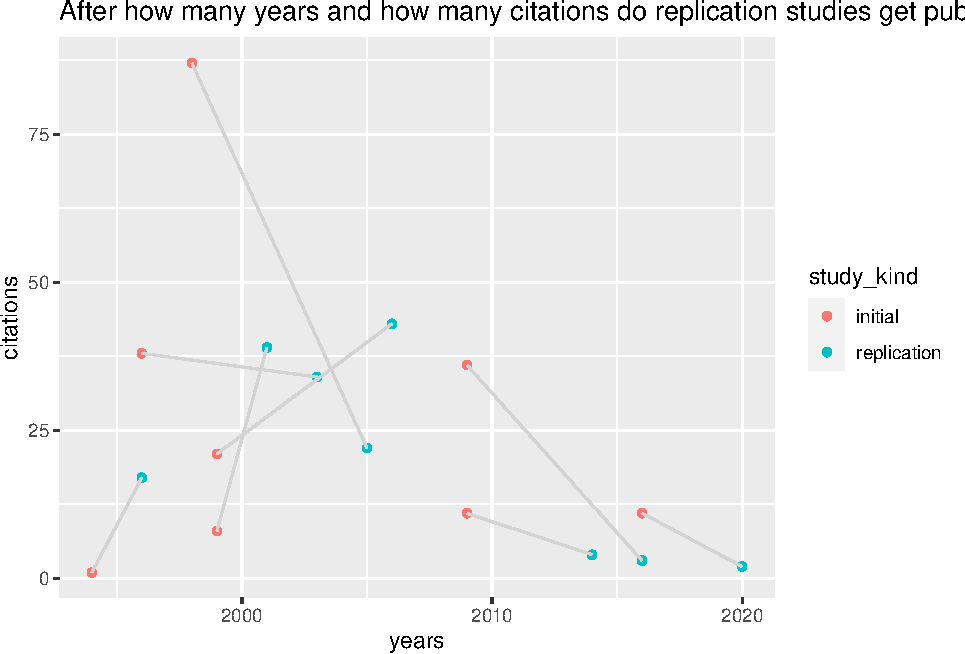
\includegraphics{ReplicationLing_files/figure-latex/plot cit and years direct-1.pdf}
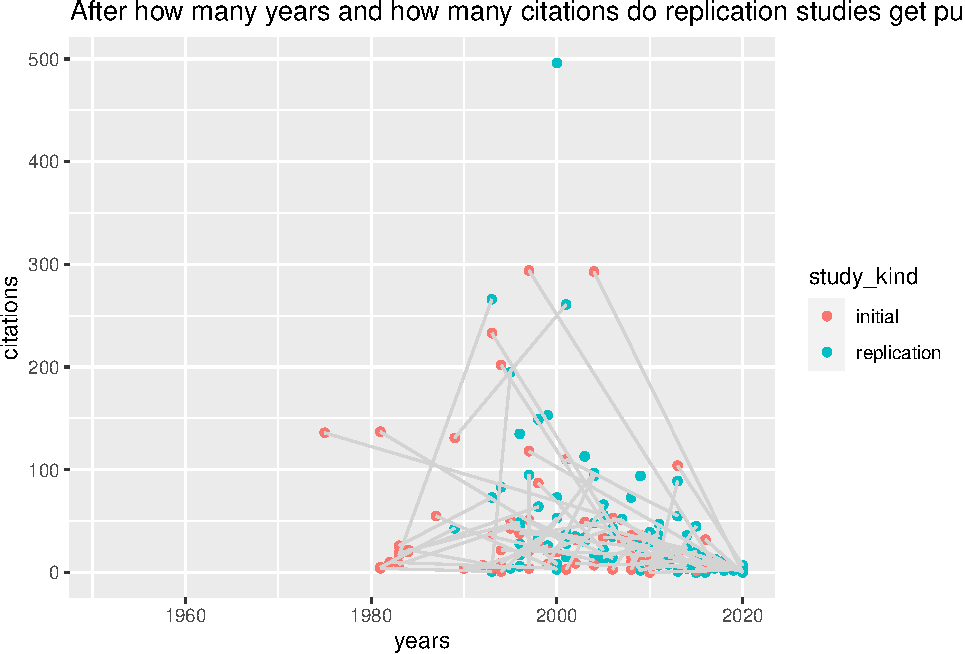
\includegraphics{ReplicationLing_files/figure-latex/plot cit and years all-1.pdf}

\begin{Shaded}
\begin{Highlighting}[]
\CommentTok{\# having a closer look at jml}
\NormalTok{jml\_data }\OtherTok{\textless{}{-}}\NormalTok{ coded\_articles }\SpecialCharTok{\%\textgreater{}\%} 
  \FunctionTok{filter}\NormalTok{(journal }\SpecialCharTok{==} \StringTok{"JOURNAL OF MEMORY AND LANGUAGE"}\NormalTok{)}

\DocumentationTok{\#\# how many really experimental}
\NormalTok{jml\_exp }\OtherTok{\textless{}{-}}\NormalTok{ jml\_data }\SpecialCharTok{\%\textgreater{}\%} 
  \FunctionTok{filter}\NormalTok{(experimental }\SpecialCharTok{==} \StringTok{"1"}\NormalTok{) }
\NormalTok{jml\_exp\_ratio }\OtherTok{=} \FunctionTok{count}\NormalTok{(jml\_exp)}\SpecialCharTok{/}\FunctionTok{count}\NormalTok{(jml\_data) }
\CommentTok{\# {-}{-}{-}\textgreater{} 50 = 100\%}

\DocumentationTok{\#\# of those how many actual replications}
\NormalTok{jml\_reps }\OtherTok{\textless{}{-}}\NormalTok{ jml\_exp }\SpecialCharTok{\%\textgreater{}\%} 
  \FunctionTok{filter}\NormalTok{(replication }\SpecialCharTok{==} \StringTok{"1"}\NormalTok{)}
\NormalTok{jml\_rep\_ratio }\OtherTok{=} \FunctionTok{count}\NormalTok{(jml\_reps)}\SpecialCharTok{/}\FunctionTok{count}\NormalTok{(jml\_exp)}
\CommentTok{\# {-}{-}{-}\textgreater{} 34 = 68\%}

\DocumentationTok{\#\# of those what types of replications}
\FunctionTok{round}\NormalTok{(}\FunctionTok{xtabs}\NormalTok{(}\SpecialCharTok{\textasciitilde{}}\NormalTok{type\_replication, jml\_reps) }\SpecialCharTok{/} \FunctionTok{nrow}\NormalTok{(jml\_reps), }\DecValTok{2}\NormalTok{)}
\end{Highlighting}
\end{Shaded}

\begin{verbatim}
## type_replication
##            conceptual     direct    partial 
##       0.00       0.44       0.09       0.47
\end{verbatim}

\begin{Shaded}
\begin{Highlighting}[]
\DocumentationTok{\#\#\# 0.44 conceptual}
\DocumentationTok{\#\#\# 0.09 direct {-}{-}\textgreater{} compared to 7\% over all journals}
\DocumentationTok{\#\#\# 0.47 partial}

\DocumentationTok{\#\# of those author overlap}
\FunctionTok{round}\NormalTok{(}\FunctionTok{xtabs}\NormalTok{(}\SpecialCharTok{\textasciitilde{}}\NormalTok{type\_replication }\SpecialCharTok{+}\NormalTok{ auth\_overlap, jml\_reps) }\SpecialCharTok{/} \FunctionTok{nrow}\NormalTok{(jml\_reps), }\DecValTok{2}\NormalTok{)}
\end{Highlighting}
\end{Shaded}

\begin{verbatim}
##                 auth_overlap
## type_replication    0    1
##                  0.00 0.00
##       conceptual 0.18 0.26
##       direct     0.06 0.03
##       partial    0.24 0.24
\end{verbatim}

\begin{Shaded}
\begin{Highlighting}[]
\DocumentationTok{\#\#\#            no   yes }
\DocumentationTok{\#\#\# conceptual 0.18 0.26}
\DocumentationTok{\#\#\# direct     0.06 0.03}
\DocumentationTok{\#\#\# partial    0.24 0.24}

\CommentTok{\# all journals:}
\DocumentationTok{\#\#\#            no   yes }
\DocumentationTok{\#\#\# conceptual 0.26 0.30}
\DocumentationTok{\#\#\# direct     0.03 0.04}
\DocumentationTok{\#\#\# partial    0.15 0.21}

\DocumentationTok{\#\# overall direct independent replication rate }
\FunctionTok{round}\NormalTok{(}\FunctionTok{nrow}\NormalTok{(jml\_data[jml\_data}\SpecialCharTok{$}\NormalTok{replication }\SpecialCharTok{==} \DecValTok{1} \SpecialCharTok{\&}
\NormalTok{                jml\_data}\SpecialCharTok{$}\NormalTok{type\_replication }\SpecialCharTok{==} \StringTok{"direct"} \SpecialCharTok{\&}
\NormalTok{                jml\_data}\SpecialCharTok{$}\NormalTok{auth\_overlap }\SpecialCharTok{==} \DecValTok{0}\NormalTok{,]) }\SpecialCharTok{/} \FunctionTok{nrow}\NormalTok{(jml\_data), }\DecValTok{3}\NormalTok{)}
\end{Highlighting}
\end{Shaded}

\begin{verbatim}
## [1] 0.04
\end{verbatim}

\begin{Shaded}
\begin{Highlighting}[]
\DocumentationTok{\#\#\# 0.04 = 4\% compared to 0.015 = 1,5\%}
\end{Highlighting}
\end{Shaded}

\hypertarget{discussion}{%
\section{Discussion}\label{discussion}}

\hypertarget{appendices}{%
\section{Appendices}\label{appendices}}

identified as A, B, etc.

\hypertarget{bibliography-styles}{%
\section{Bibliography styles}\label{bibliography-styles}}

There are various bibliography styles available. You can select the
style of your choice in the preamble of this document. These styles are
Elsevier styles based on standard styles like Harvard and Vancouver.
Please use BibTeX~to generate your bibliography and include DOIs
whenever available.

Here are two sample references: (Dirac, 1953; Feynman and Vernon Jr.;
1963).

\hypertarget{references}{%
\section*{References}\label{references}}
\addcontentsline{toc}{section}{References}

\hypertarget{refs}{}
\begin{CSLReferences}{1}{0}
\leavevmode\vadjust pre{\hypertarget{ref-Dirac1953888}{}}%
Dirac, P.A.M., 1953. The lorentz transformation and absolute time.
Physica 19, 888--896.
doi:\href{https://doi.org/10.1016/S0031-8914(53)80099-6}{10.1016/S0031-8914(53)80099-6}

\leavevmode\vadjust pre{\hypertarget{ref-Feynman1963118}{}}%
Feynman, R.P., Vernon Jr., F.L., 1963. The theory of a general quantum
system interacting with a linear dissipative system. Annals of Physics
24, 118--173.
doi:\href{https://doi.org/10.1016/0003-4916(63)90068-X}{10.1016/0003-4916(63)90068-X}

\end{CSLReferences}


\end{document}
